\documentclass[12pt]{report}
\usepackage[utf8]{inputenc}
\usepackage[none]{hyphenat} %Para evitar el corte de palabras
\usepackage{amsmath}
\usepackage{amsthm} %Para definir ambientes con \newtheorem
\usepackage{amsfonts}
\usepackage{amssymb}
\usepackage{makeidx}
\usepackage{graphicx}
\usepackage[square,sort,comma,numbers]{natbib}
\usepackage{url}
%\usepackage{titlesec}
%\usepackage{float}

\bibliographystyle{elsarticle-harv}

\title{Aprendizaje de reglas para operaciones en el mercado accionario}
%\publishers{Centro de Investigación en Computación, Instituto Politécnico Nacional}
\date{}
\author{David Ricardo Montalván Hernández}
	
%=========Define los ambientes a utilizar =======%
%Define estilo para dar un salto de línea en el encabezado
%del 'teorema'
\newtheoremstyle{break}
{2ex} %above space
{2ex} %below space
{} %Body font \itshape)
{} %indent amount
{\bfseries} %head font
{:} %post head puncuation
{\newline} %post head space
{}

\theoremstyle{break}
%Definición
\newtheorem{definicion}{Definición}[chapter]

%Teorema
\newtheorem{teorema}{Teorema}[chapter]

%Notas importantes
\newtheorem{nota}{Nota}[chapter]

%Algoritmo (Utiliza el ambiente tabbing)
\theoremstyle{break}
\newtheorem{algoritmo}{Algoritmo}[chapter]
%=================================================%

%====================Macros=======================%
%\newcommand{\buyhold}{\textit{compra y espera}}
%=================================================%

\begin{document}
\sloppy %Para justificar correctamente (tiene que ver con \usepackage[none]{hyphenat})
\maketitle
\pagenumbering{Roman} %numeración romana con mayúsculas

\chapter*{Dedicatoria}
A mis padres y amigos.

\chapter*{Agradecimientos}
Agradezco a mi director de tesis el doctor Salvador Godoy Calderón por su apoyo en la realización de este trabajo.

Agradezco también a cada uno de los miembros de mi comité tutorial por sus valiosas observaciones.

\renewcommand{\contentsname}{Contenido}
\tableofcontents
\renewcommand{\listfigurename}{Lista de figuras}
\listoffigures
\renewcommand{\listtablename}{Lista de tablas}
\renewcommand\tablename{Tabla}
\renewcommand{\bibname}{Referencias}
\renewcommand{\figurename}{Figura}
\renewcommand{\chaptername}{Capítulo}
\listoftables

\chapter*{Resumen}
El incremento en el poder de cómputo, la digitalización de los mercados financieros y la oportunidad de obtener grandes ganancias, son algunos de los factores que han motivado la investigación y desarrollo de algoritmos computacionales enfocados a guiar la toma de decisiones de inversión. En particular, se busca que estos algoritmos sean capaces de determinar los momentos adecuados para realizar compras o ventas de un activo financiero.

En este trabajo se propone una metodología para aprender, de manera automática, un conjunto de reglas de la forma \textit{si...entonces}, las cuales nos permitirán generar un conjunto de estrategias de inversión. Estas estrategias serán probadas utilizando datos del mercado accionario mexicano y estadounidense.

Además, desde el punto de vista de la teoría económica, este trabajo investiga la hipótesis del mercado eficiente en su versión débil.

\chapter*{Abstract}
The increase in the computing power, the digitalization of financial markets and the opportunity of making big profits, are among the factors that have influenced the research and development of computational algorithms whose objective is to guide the investment decisions process. Concretely, these algorithms should be able to determine when is the right moment to buy or sell a financial asset.

In this work, a methodology for automatically learning a set of \textit{If...then} rules that will allow us to generate a set of trading strategies is proposed. These strategies will be tested using data from the Mexican and American stock market.

Added to this, from the point of view of economic theory, this work investigates the weak version of the efficient market hypothesis.

%\chapter*{The modeler's hippocratic oath}
%\begin{itemize}
%\item I will remember that I didn’t make the world, and it doesn’t satisfy my equations.
%\item Though I will use models boldly to estimate value, I will not be overly impressed by mathematics.
%\item I will never sacrifice reality for elegance without explaining why I have done so.
%\item Nor will I give the people who use my model false comfort about its accuracy. Instead, I will make explicit its assumptions and oversights.
%\item I understand that my work may have enormous effects on society and the economy, many of them beyond my comprehension.
%\end{itemize}

%\begin{center}
%\textit{Paul Wilmott y Emmanuel Derman.}
%\end{center}

%=============== INTRODUCCIÓN ================= %
\chapter[Capítulo \thechapter: Introducción]{Introducción}
\pagenumbering{arabic} %Numeración árabe
\label{capitulo:introduccion}
%Motivación y ¿qué es lo que se busca con este trabajo?
%Objetivo general y objetivos particulares.
%Estructura del trabajo.
El incremento en el poder de cómputo, la digitalización de los mercados financieros y la oportunidad de obtener grandes ganancias, son algunos de los factores que han motivado la investigación y desarrollo de algoritmos computacionales enfocados a guiar la toma de decisiones de inversión, en particular, determinar los momentos adecuados para realizar compras o ventas de instrumentos financieros.

A pesar de que la idea básica es comprar barato y vender caro, la incertidumbre y complejidad de los mercados financieros han dado lugar al uso de herramientas computacionales con el fin de guiar la toma de decisiones, concretamente, técnicas relacionadas al aprendizaje de máquina han ganado notoriedad \cite{AdvancesMLFinance}.

El objetivo general de este trabajo es proponer una metodología para aprender, de manera automática, un conjunto de reglas \textit{si...entonces}. Estas reglas se utilizarán para obtener estrategias de inversión cuya ganancia, buscamos, sea superior a la ganancia generada por la estrategia de \textit{compra y espera}, la cual es usada comúnmente como una estrategia de referencia (ver sección \ref{seccion:mercado eficiente}).

Además, la metodología propuesta busca obtener un modelo interpretable, contrastando con la tendencia actual que se caracteriza por el uso de las llamadas \textit{cajas negras}, por ejemplo redes neuronales (ver sección \ref{capitulo:antecedentes}).

Los objetivos particulares de este trabajo son:
\begin{itemize}

\item Selección de las fuentes de datos.

\item Proponer una metodología para etiquetar los datos y así poder aplicar algoritmos de aprendizaje supervisado.

\item Seleccionar la forma de separar los conjuntos de entrenamiento y prueba.

\item Proponer una metodología para aplicar un aprendizaje incremental. Esta metodología permitirá que el modelo aprenda de los errores cometidos.
\end{itemize}

La estructura de este trabajo es la siguiente:

En la sección \ref{capitulo:antecedentes}, se dan los antecedentes del problema y se exploran las distintas metodologías que han sido empleadas con el fin de generar estrategias de inversión. Se hace un análisis comparativo entre los enfoques utilizados así como los tipo de mercado analizados.

En la sección \ref{capitulo:marco teorico}, se da un panorama general sobre el funcionamiento de los mercados de índices accionarios, se explica la hipótesis del mercado eficiente así como sus posibles versiones y el tipo de información relacionada a cada una de ellas. Se explica la estrategia \textit{compra y espera} y la métrica de desempeño que se utilizará para evaluar nuestras estrategias. En la sección \ref{subseccion:indicadores tecnicos} se explican los atributos que se utilizarán y en la sección \ref{seccion:algoritmos aq cn2} los algoritmos de inducción de reglas utilizados.

En la sección \ref{capitulo:solucion propuesta}, se explican los datos utilizados y la metodología propuesta, se establece además, la metodología de etiquetado y la forma de separar los conjuntos de entrenamiento y prueba. Finalmente se explica la forma en que se realiza el aprendizaje incremental propuesto, así como los supuestos bajo los cuales se trabajó.

La sección \ref{capitulo:resultados experimentales} contiene los resultados experimentales de cada uno de los experimentos.

Para finalizar, la sección \ref{capitulo:conclusiones} trata las conclusiones obtenidas así como las posibles direcciones para extender este trabajo.

\section{Contribuciones}
\label{seccion:contribuciones}
Una de las principales contribuciones es el análisis del mercado accionario mexicano desde una enfoque basado en reglas. El análisis del estado del arte indica que esta es la primera vez que se analiza este mercado utilizando dicho enfoque.

%=============== Antecedentes ================= %
\chapter[Capítulo \thechapter: Revisión del estado del arte]{Revisión del estado del arte}
\label{capitulo:antecedentes}
%orden cronológico
%Tabla con referencia, mercado, metodologia
%Tabla con referencia, vence bh, considera costos de transacción
Al analizar el estado del arte, se puede observar que las heurísticas evolutivas juegan un papel esencial para obtener las reglas con las cuales se opera en el mercado. Además, los atributos utilizados en la mayoría de los trabajos son un conjunto de indicadores técnicos (ver sección \ref{subseccion:indicadores tecnicos}).

Las tablas \ref{tabla:referencia-mercado-tecnica} y \ref{tabla:referencia-venceBH} muestran un resumen del estado del arte recolectado para este trabajo, como se puede observar existen resultados mixtos respecto a la estrategia \textit{compra y espera}, que comúnmente es utilizada como estrategia de referencia.

Uno de los primeros artículos en donde se utilizan técnicas relacionadas al aprendizaje de reglas es \cite{Allen1999}, en este trabajo se utiliza una metodología basada en programación genética, obteniéndose de esta manera un conjunto de reglas \textit{si...entonces}, para operar en el mercado. Los autores analizan el mercado accionario de Estados Unidos utilizando la información del índice accionario S\&P 500 (ver sección \ref{seccion:indices accionarios}) y comparándose contra la estrategia \textit{compra y espera} (ver sección \ref{seccion:buy and hold}) obteniendo resultados poco favorables.

En \cite{Leigh2002}, se utiliza un enfoque basado en empate de patrones (template match) a partir del cual se obtienen un conjunto de reglas \textit{si...entonces}. Esta metodología se basa en detectar patrones en las gráficas de los precios, concretamente, se busca el patrón llamado \textit{bull flag} el cual es considerado como un patrón que indica el inicio de una tendencia a la alza en los precios. Este artículo utiliza la estrategia \textit{compra y espera} como referencia, obteniendo mayores ganancias que ésta, sin embargo, cabe señalar que no se consideran costos de transacción\footnote{Se entiende por costos de transacción, a las comisiones que se cobran por realizar una compra o una venta.}, por lo que la metodología se vuelve poco realista. El mercado analizado es el mercado de Estados Unidos a través del índice accionario NYSE Composite.

Los autores en \cite{Potvin2004}, retoman el trabajo de \cite{Allen1999} modificando la forma en que se crean los árboles y considerando $14$ compañías canadienses que forman parte del índice accionario TSE $300$. A pesar de que vencen a la estrategia \textit{compra y espera} en $9$ de las $14$ compañías, no se consideran costos de transacción.

En \cite{Parracho2010}, se retoma el trabajo de \cite{Leigh2002} introduciendo un algoritmo genético para realizar un proceso de optimización sobre parámetros que antes se consideraban fijos. Se obtienen resultados favorables pero sin considerar costos de transacción.

Una línea totalmente distinta a los artículos anteriores es el trabajo de \cite{Kaucic2010}. En este, no se busca obtener un conjunto de reglas \textit{si...entonces}, si no que busca encontrar, a través de un aprendizaje evolutivo, la mejor combinación de indicadores técnicos (ver sección \ref{seccion:analisisTecnico}) con la cual se busca determinar los momentos adecuados para comprar o vender. Únicamente se logra vencer a la estrategia \textit{compra y espera} en mercados a la baja o estables (considerando costos de transacción). Se analiza el mercado accionario de Estados Unidos.

Los trabajos \cite{Allen1999} y \cite{Potvin2004}, se retoman en \cite{Lohpetch2010}, en donde no sólo se usan precios diarios, si no que también se utilizan precios semanales y mensuales, además, en el proceso evolutivo que crea los árboles, se utiliza una función de aptitud que penaliza la complejidad de estos, evitando así un sobre ajuste en los datos de entrenamiento. En este trabajo se logra vencer a la estrategia \textit{compra y espera} (utilizando el exceso de ganancia como medida de desempeño, ver sección \ref{subseccion:exceso de ganancia}) aún considerando costos de transacción.

En \cite{Teixeira2010}, se logra vencer a la estrategia \textit{compra y espera} (considerando costos de transacción) utilizando una metodología basada en el algoritmo \textit{k nearest neighbors} (K-NN). Se analizan $15$ series accionarias pertenecientes al mercado brasileño. Una propuesta interesante de este artículo, es el uso de límites que capturan el perfil de riesgo de los inversionistas\footnote{En finanzas estos límites son llamados stop loss y take profits} (ver sección \ref{seccion:limites ventas}).

La serie de artículos \cite{Canelas2012-gecco}, \cite{Canelas2013-gecco}, \cite{Canelas2013-journal}, \cite{Leitao2016}; desarrolla una metodología en la cual se busca reducir la dimensión de la serie de tiempo al identificar los llamados "puntos perceptualmente importantes" (perceptually important points, PIPs). Una vez identificados estos puntos, se calcula la variación porcentual entre ellos y de acuerdo a esta cantidad la serie de tiempo es convertida en una cadena de símbolos. Estos símbolos son comparados con un patrón base obtenido a través de un algoritmo genético y de acuerdo a esta comparación se obtienen las señales de compra. Se vence a la estrategia \textit{compra y espera} pero no se consideran costos de transacción.

En \cite{Hu2015-XCS}, se utiliza aprendizaje por reforzamiento junto con un algoritmo evolutivo para obtener un conjunto de reglas \textit{si..entonces}.\footnote{Extended Classifier System, XCS} Estas reglas son aplicadas para operar en el mercado de índices accionarios de la bolsa de Shangai, se vence a la estrategia \textit{compra y espera} aún considerando costos de transacción.

\begin{center}
\begin{table}[htbp]
\centering
\begin{tabular}{ccc}
\hline
\textbf{Referencia} & \textbf{Mercado} & \textbf{Técnica} \\
\hline
\cite{Allen1999} & Estados Unidos & Programación genética \\
\cite{Leigh2002} & Estados Unidos & Emparejamiento de patrones\\
\cite{Potvin2004} & Canadá & Programación genética\\
\cite{Parracho2010} & Estados Unidos & Emparejamiento de patrones\\
\cite{Kaucic2010} & Estados Unidos & Aprendizaje evolutivo\\
\cite{Lohpetch2010} & Estados Unidos & Programación genética\\
\cite{Teixeira2010} & Brasil & K-NN\\
\cite{Preen2010} & Estados Unidos & Aprendizaje evolutivo\\
\cite{Esfahanipour2011} & Irán & Programación genética\\
\cite{Canelas2012-gecco}, \cite{Canelas2013-gecco}, \cite{Canelas2013-journal}, \cite{Leitao2016} & Estados Unidos & PIP-SAX \\
\cite{Kuo2013} & Taiwan & Búsqueda tabú \\
\cite{Wang2014} & Estados Unidos & Enjambre de partículas \\
\cite{Hu2015-XCS} & Shangai & XCS \\
\cite{Huang2015} & Varios & Biagrupamiento \\
\cite{Kim2016} & Corea & Conjuntos rugosos \\
\cite{Kampouridis2017} & Tipo de cambio & Aprendizaje evolutivo\\
\cite{Sezer2017} & Estados Unidos & Redes neuronales\\
\cite{Alimoradi2018} & Irán & Q-learning\\
\hline
\end{tabular}
\caption{\label{tabla:referencia-mercado-tecnica} Comparativo del estado del arte por mercado y técnica utilizada}
\end{table}
\end{center}

\begin{center}
\begin{table}[htbp]
\centering
\begin{tabular}{ccc}
\hline
\textbf{Referencia} & \textbf{Vence \textit{compra y espera}} & \textbf{Considera costos de transacción} \\
\hline
\cite{Allen1999} & No & Si \\
\cite{Leigh2002} & Si & No\\
\cite{Potvin2004} & Si (periodos estables o a la baja)  & No\\
\cite{Parracho2010} & Si & No\\
\cite{Kaucic2010} & Si (periodos estables o a la baja) & Si\\
\cite{Lohpetch2010} & Si & Si\\
\cite{Teixeira2010} & Si & Si\\
\cite{Preen2010} & Si (mayoría de los casos) & Si\\
\cite{Esfahanipour2011} & Si & Si\\
\cite{Canelas2012-gecco}, \cite{Canelas2013-gecco}, \cite{Canelas2013-journal}, \cite{Leitao2016} & Si & No \\
\cite{Kuo2013} & Si & Si \\
\cite{Wang2014} & No hay comparación & Si \\
\cite{Hu2015-XCS} & Si & Si \\
\cite{Huang2015} & Si & No \\
\cite{Kim2016} & Si & No \\
\cite{Kampouridis2017} & Si & Si\\
\cite{Sezer2017} & Resultados mixtos & Si\\
\cite{Alimoradi2018} & Si & Si\\
\hline
\end{tabular}
\caption{\label{tabla:referencia-venceBH} Comparativo del estado del arte por desempeño respecto a la estrategia \textit{compra y espera}}
\end{table}
\end{center}


%=============== Marco teórico ================= %
\chapter[Capítulo \thechapter: Marco teórico]{Marco teórico}
\label{capitulo:marco teorico}

\section{Mercado de índices accionarios}
\label{seccion:indices accionarios}

Se inicia esta sección con algunas definiciones básicas \cite{CFA2019-market-org}.

\begin{definicion}[Mercado]
\label{definicion:mercado}
Un mercado es un lugar en donde dos partes se reúnen para realizar el intercambio de bienes o servicios.
\end{definicion}

\begin{definicion}[Acciones]
\label{definicion:instrumento-financiero}
Un \textbf{instrumento financiero} es un contrato monetario entre dos partes. Si este contrato da derechos de propiedad sobre los activos de una compañía, entonces recibe el nombre de \textbf{acción}.
\end{definicion}

\begin{definicion}[Mercado financiero]
\label{definicion:mercado-financiero}
Un mercado financiero es un mercado en el cual se intercambian instrumentos financieros, por ejemplo acciones.
\end{definicion}

Debido a la diversidad de los tipos de mercados financieros (accionario, deuda, tipo de cambio, derivados, etc.) así como al funcionamiento particular de cada uno de ellos, fue necesario restringir este estudio a un mercado en particular. Siendo concretos, este trabajo únicamente analiza el mercado de índices accionarios.

\begin{definicion}[Índice accionario]
\label{definicion:indice-accionario}
Un índice accionario, busca representar el comportamiento de un segmento específico del mercado financiero accionario, por ejemplo un sector o un área geográfica en particular \cite{CFA2019-market-index}.
\end{definicion}

Así pues, el propósito principal de este tipo de índices es representar la opinión colectiva que se tiene respecto a un conjunto de acciones.

En este trabajo consideraremos lo siguientes índices :

\begin{itemize}
\item Índice de precios y cotizaciones (S\&P/BMV IPC)
\item Índice Standard and Poors 500 (S\&P 500)
\end{itemize}

El índice de precios y cotizaciones es el principal indicador del mercado accionario mexicano. Este índice busca medir el desempeño de las acciones listadas en la Bolsa Mexicana de Valores utilizando una muestra con las 35 series accionarias de mayor tamaño y liquidez listadas en dicha bolsa\footnote{https://espanol.spindices.com/indices/equity/sp-bmv-ipc}.

Por otro lado, el índice Standard and Poors 500 es considerado como el mejor indicador para el mercado accionario de Estados Unidos. Este índice está compuesto por las 500 empresas de mayor capitalización las cuales capturan alrededor del $80\%$ de la capitalización del mercado\footnote{https://us.spindices.com/indices/equity/sp-500}

\begin{nota} \label{nota:ETF}
En la práctica los inversionistas no pueden comprar los índices accionarios, en cambio, los instrumentos negociados reciben el nombre de Títulos Referenciados a Acciones (TRACS\footnote{En inglés Exchange Traded Funds o ETF}). Estos instrumentos buscan replicar el comportamiento del índice al que están relacionados.

El instrumento que busca replicar el índice de precios y cotizaciones recibe el nombre de iShares NAFTRAC (o simplemente NAFTRAC), mientras que para el índice Standard and Poors 500 el instrumento relacionado es el SPDR S\&P 500.
\end{nota}

\section{Mercado eficiente}
\label{seccion:mercado eficiente}
El concepto de mercado eficiente, hace a un mercado que es capaz de capturar, de forma rápida y precisa, la información\footnote{Información relacionada a la economía en general.} disponible más reciente. Esta información es reflejada en los precios de los instrumentos financieros y como consecuencia, en un mercado eficiente, los precios son informativos, lo que permite lograr una colocación eficiente de los recursos (ver \cite{Fama1965} y \cite{CFA2019}).

\subsection{Versiones de eficiencia en el mercado}
\label{subseccion:versiones emh}
Eugene Fama describe tres formas de eficiencia de un mercado: débil, semifuerte y fuerte \cite{Fama1965}.

En la versión débil, los precios actuales reflejan toda la información histórica del mercado, es decir, la información del pasado relativa a precios y al volumen negociado. En consecuencia, bajo esta versión de eficiencia, no es posible utilizar datos históricos con el fin de predecir la tendencia futura de los precios (ver sección \ref{seccion:analisisTecnico}).

La versión semifuerte incluye la versión débil y añade que, además de reflejar la información histórica del mercado, los precios actuales reflejan toda la información pública. La información pública es aquella a la cual el público inversionista puede acceder, por ejemplo, noticias económicas o financieras, estados de resultados de las empresas, reportes anuales o trimestrales de las mismas, indicadores macroeconómicos etc. De acuerdo a esta versión, no es posible utilizar dicha información con el fin de predecir la tendencia futura de los precios.

Finalmente, la versión fuerte de la eficiencia de un mercado, nos dice que los precios actuales reflejan totalmente tanto la información pública como la información privada, es decir, aquella que solamente algunas personas poseen. Por lo tanto, bajo esta versión, incluso tomando en cuenta la información privada, no es posible predecir la tendencia futura de los precios.

Por lo tanto, la eficiencia de un mercado debe ser interpretada relativa al tipo de información que los inversionistas utilizan. Además, como se señala en \cite{CFA2019}, la eficiencia cae en un espectro continuo, que varía a través del tiempo, regiones geográficas y tipo de mercado.

La figura \ref{imagen:versiones emh} ilustra las distintas versiones de la eficiencia de un mercado.

Este trabajo se enfoca únicamente en la versión débil de la eficiencia de un mercado.

\begin{figure}[ht]
\centering
\scalebox{0.8}{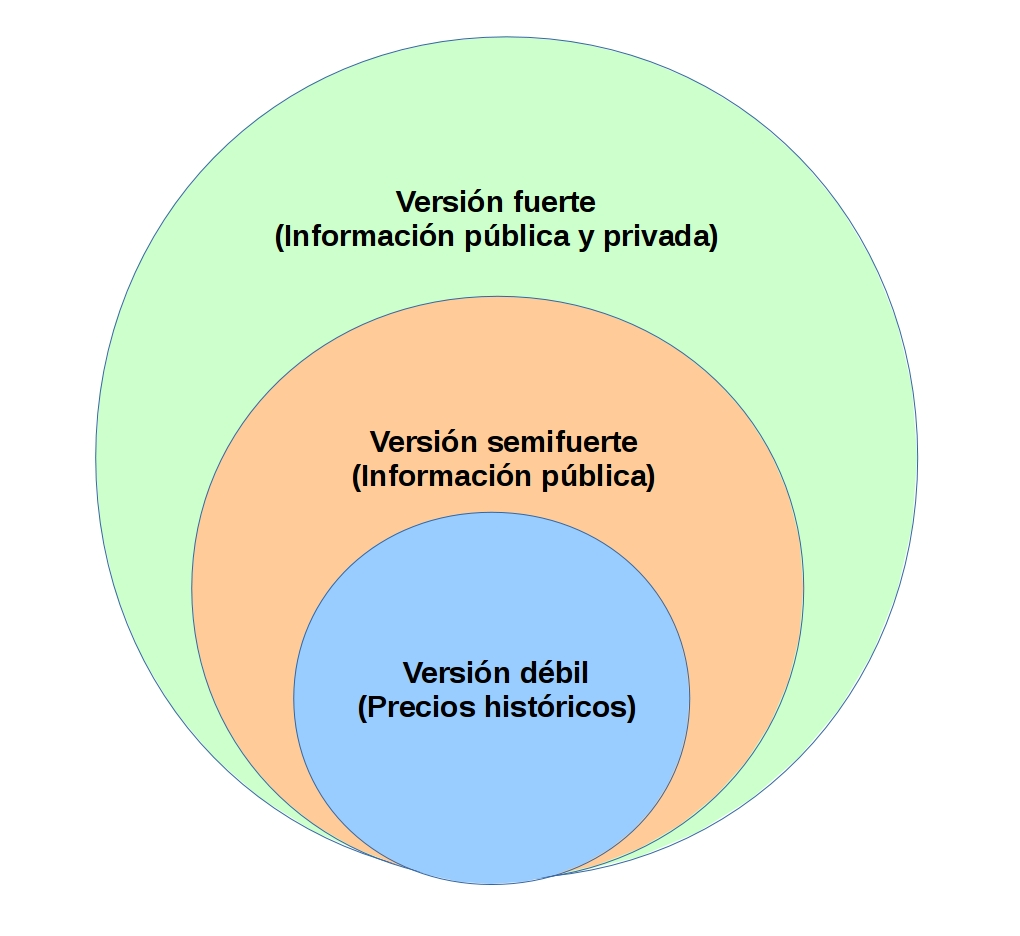
\includegraphics[width=.8\linewidth]{imagenes/versiones-emh.jpeg}}
\caption{\label{imagen:versiones emh} Versiones de la eficiencia de un mercado}
\end{figure}


\subsection{Estrategia \textit{compra y espera}}
\label{seccion:buy and hold}
Como se señala en la sección \ref{subseccion:versiones emh}, de acuerdo a la hipótesis del mercado eficiente, no es posible utilizar información histórica con el fin de predecir los precios del futuro. Lo mejor que se puede hacer es comprar un portafolio bien diversificado y mantenerlo por un periodo de tiempo predeterminado, esta estrategia recibe el nombre de estrategia \textit{compra y espera}.

De acuerdo a lo anterior se tiene que, en un mercado eficiente, no es posible obtener, de manera consistente y sistemática, ganancias superiores a aquellas generadas por la estrategia \textit{compra y espera}.

Dado un plazo de tiempo fijo, $\left[T_{I}, T_{F}\right]$, la ganancia de la estrategia \textit{compra y espera} está dada por la ecuación (\ref{eqn:ganancia BH})

\begin{equation} \label{eqn:ganancia BH}
G_{\left[T_{I}, T_{F}\right]} (BH) = \dfrac{P_{T_F} (1 - c) } { P_{T_I} (1 + c) } - 1
\end{equation}

en donde $P_{T_F}$ es el precio de ejecución al final del plazo, $P_{T_I}$ es el precio de ejecución al inicio de este y $c$ es el costo (porcentual) de cada transacción, es decir, la comisión que se debe de pagar por ejecutar la transacción (ver sección \ref{sec:supuestos del mercado}). 

La figura \ref{imagen:buy hold alza} ejemplifica la estrategia \textit{compra y espera} en un periodo en el cual el mercado presenta una tendencia a la alza. Como se puede observar, vencer esta estrategia cuando se presenta este tipo de tendencia es todo un reto, esto se debe a que sólo se involucran dos operaciones, lo que implica un ahorro en costos de transacción.

\begin{figure}[ht]
\centering
\scalebox{0.8}{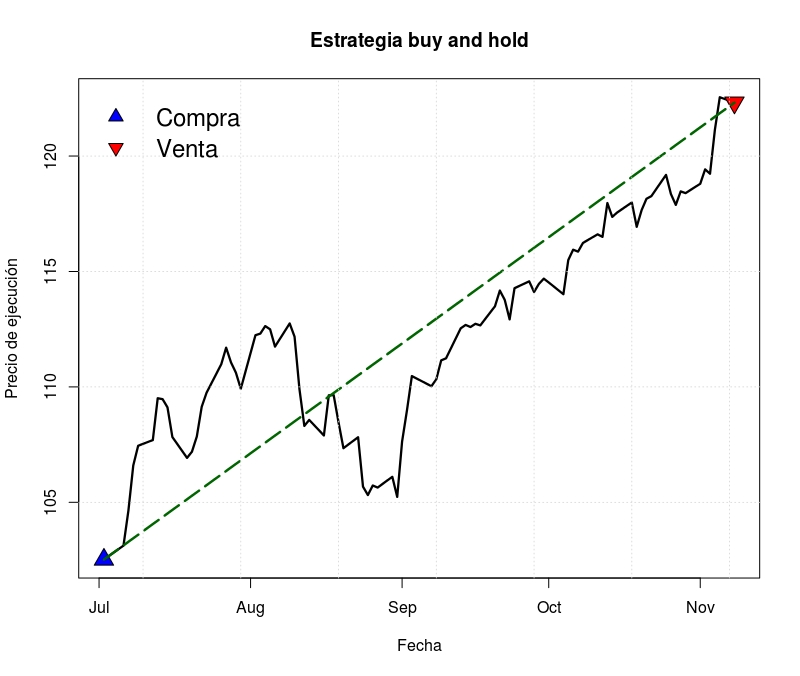
\includegraphics[width=1\linewidth]{imagenes/buy-hold-alza.jpeg}}
\caption{\label{imagen:buy hold alza} Estrategia \textit{compra y espera} en un mercado a la alza}
\end{figure}

\subsection{Exceso de ganancia sobre compra y espera}
\label{subseccion:exceso de ganancia}

Para comparar las estrategias propuestas en este trabajo contra la estrategia \textit{compra y espera}, se utiliza como métrica de desempeño el exceso de ganancia (porcentual).

Esta métrica compara la ganancia obtenida por una estrategia, $S$, con aquella obtenida por la estrategia \textit{compra y espera}.

\begin{definicion}[Exceso de ganancia]
\label{definicion:exceso de ganancia}
Para un plazo fijo, $\left[T_{I}, T_{F}\right]$, el exceso de ganancia de una estrategia $S$, sobre la estrategia \textit{compra y espera}, está dado por la ecuación (\ref{eqn:Exceso de ganancia})

\begin{equation} \label{eqn:Exceso de ganancia}
ExG_{\left[T_{I}, T_{F}\right]} = G_{\left[T_{I}, T_{F}\right]} (S) - G_{\left[T_{I}, T_{F}\right]} (BH)
\end{equation}

en donde la ganancia $G_{\left[T_{I}, T_{F}\right]} (BH)$, está dada por la ecuación (\ref{eqn:ganancia BH}) y la ganancia $G_{\left[T_{I}, T_{F}\right]} (S)$ es simplemente la variación porcentual entre el capital inicial disponible en el momento $T_{I}$ y el capital con el que se cuenta en el momento $T_{F}$.

\begin{equation} \label{eqn:Ganancia estrategia S}
G_{\left[T_{I}, T_{F}\right]}(S) = \dfrac{Capital_{T_F}}{Capital_{T_I} } - 1 
\end{equation}
\end{definicion}
Claramente buscamos que $ExG_{\left[T_{I}, T_{F}\right]}$ sea un número positivo.

\section{Análisis técnico}
\label{seccion:analisisTecnico}
Contrario a lo que establece la hipótesis del mercado eficiente (sección \ref{seccion:mercado eficiente}), el análisis técnico busca predecir la tendencia futura en los precios utilizando la información histórica del mercado (precios y volumen) \cite{murphy1999technical}.

Los tres supuestos en los que se basa este tipo de análisis son los siguientes:

\begin{itemize}
\item La información de todos los factores que afectan a la oferta y a la demanda se encuentra reflejada en el precio de los instrumentos financieros. En consecuencia, basta centrarse en el estudio de los precios para poder analizar el mercado.

\item Los precios se mueven siguiendo tendencias (a la alza o a la baja). El objetivo del análisis técnico es detectar, lo más pronto posible, el inicio y el final de estas tendencias.

\item Los patrones en los precios tienden a repetirse.
\end{itemize}


\subsection{Indicadores técnicos}
\label{subseccion:indicadores tecnicos}
Para realizar el pronóstico de las tendencias, el análisis técnico se vale del uso de indicadores técnicos. Estos indicadores son transformaciones aplicadas a la información histórica para una ventana (deslizante) de tiempo determinada \cite{murphy1999technical}, \cite{technicalAnalysisKirkPatrick}, \cite{encycoplediaTechnicalIndicators}.

Los indicadores técnicos utilizados en este trabajo, serán\footnote{Aunque en las fórmulas no se indica, cada indicador se calcula en cada periodo $t$ utilizando la información en el intervalo $\left[t-n + 1, t\right]$, es decir, la información contenida en una ventana deslizante de tamaño $n$. }:

\begin{itemize}
\item Oscilador aroon.

\item Relative strength index (RSI).

\item Money flow index (MFI).

\item Williams \%R.

\item Commodity channel index (CCI).
\end{itemize}


\subsubsection{Oscilador aroon}
\label{subsubseccion:Oscilador Aroon}
Este indicador mide el número de periodos, dentro de una ventana de tiempo de tamaño $n$, que han transcurrido desde el máximo y el mínimo más reciente. El cálculo de este indicador está dado en la ecuación (\ref{eqn:oscilador aroon})

\begin{equation} \label{eqn:oscilador aroon}
OsAroon = 100 \left( \dfrac{  n - T_H  } { n } - \dfrac{  n - T_L  } { n } \right)
\end{equation}

en donde $n$ es el número de periodos que comprende la ventana de tiempo, $T_H$ es el número de periodos transcurridos desde el último máximo registrado dentro de la ventana de tamaño $n$ y $T_L$ es el número de periodos transcurridos desde el último mínimo registrado dentro de la ventana de tamaño $n$.

Vemos entonces que, de acuerdo a la ecuación (\ref{eqn:oscilador aroon}), si $OsAroon$ es un número positivo, los precios muestran una tendencia a la alza (debemos de prepararnos para comprar). En cambio cuando $OsAroon$ es un número negativo, los precios muestran una tendencia a la baja (debemos de prepararnos para vender).

\subsubsection{Relative strength index (RSI)}
\label{subsubseccion:RSI}
Este indicador busca predecir la tendencia en los precios analizando el promedio de ganancias y pérdidas obtenidas para una ventana de tiempo de tamaño $n$. La fórmula para calcular el RSI está dada en la ecuación (\ref{eqn:RSI})

\begin{equation} \label{eqn:RSI}
RSI = 100 - \left( \frac{100}{1 + RS} \right)
\end{equation}

en donde 

\begin{equation} \label{eqn:RSI RS}
RS = \frac{Ganancia\,promedio\,en\,n\,periodos}{P\acute{e}rdida\,promedio\,en\,n\,periodos}
\end{equation}

Típicamente, en la literatura financiera (\cite{technicalAnalysisKirkPatrick}, \cite{encycoplediaTechnicalIndicators}) una señal de venta se genera cuando $RSI > 70$; por otra parte, una señal de compra se genera si $RSI < 30$.

\subsubsection{Money flow index (MFI)}
\label{subsubseccion:money flow index}
Este indicador es similar al RSI. Considera el número de periodos en los que se han presentado ganancias o pérdidas tomando en cuenta tanto los precios como el volumen del periodo (en comparación con el RSI que sólo considera los precios).

Para el cálculo del MFI se necesita primero calcular el precio promedio del periodo $t$, el cual está dado por la ecuación (\ref{eqn:precio tipico})

\begin{equation} \label{eqn:precio tipico}
Precio\, \, promedio_t = \dfrac{H_{t} + L_{t} + C_{t}}{3}
\end{equation}

en donde $H_{t}, L_t, C_t$ representan, respectivamente, el precio máximo, mínimo y de cierre en el periodo $t$.

Una vez calculado el precio promedio, se calcula el flujo de efectivo del periodo, como se muestra en la ecuación (\ref{eqn:flujo de efectivo})

\begin{equation} \label{eqn:flujo de efectivo}
MF_t = Precio\, \, promedio_t \times Volumen_t \times F_t
\end{equation}

en donde $F_t = 1$, si el precio promedio del periodo $t$ es mayor al precio promedio del periodo $t-1$, y $F_t = -1$ en el caso contrario.

Así, dada una ventana de tiempo de tamaño $n$, el MFI se calcula de acuerdo a la ecuación (\ref{eqn:MFI})

\begin{equation} \label{eqn:MFI}
MFI = 100 - \left( \frac{100}{1 + MFR} \right)
\end{equation}

en donde $MFR$ está dado por 

\begin{equation} \label{eqn:MFR}
MFR = \dfrac{\sum_{MF_t > 0} MF_t  }{\sum_{MF_t < 0} MF_t}
\end{equation}

con $t$ dentro del periodo de la ventana $n$.

En la práctica, es común considerar que una señal de venta se da cuando $MFI > 80$, mientras que una señal de compra se da cuando $MFI < 20$.

\subsubsection{Williams \%R}
\label{subsubseccion:Williams R}
Este indicador busca reflejar el precio de cierre relativo al precio máximo dentro de una ventana de tiempo dada.

Su cálculo está dado por la ecuación (\ref{eqn:williams R})

\begin{equation} \label{eqn:williams R}
Williams \%R_t = -100 \times \dfrac{HH - C_t}{HH - LL}
\end{equation}

en donde $HH$ es el máximo entre los precios máximos de cada periodo que comprende la ventana de tiempo, de manera similar $LL$ es el mínimo de los precios mínimos de cada periodo en la ventana de tiempo y $C_t$ es el precio de cierre en el tiempo $t$.

Se considera típicamente que si este indicador se encuentra entre $0$ y $-20$, es un momento apropiado para vender, mientras que si se encuentra dentro del rango de $-80$ a $-100$, es un momento adecuado para comprar.

\subsubsection{Commodity channel index (CCI)}
\label{subsubseccion:cci}
Este indicador mide la diferencia entre el precio promedio en el periodo $t$ (como se define en la ecuación (\ref{eqn:precio tipico})) y un promedio móvil de este mismo precio utilizando una ventana de tiempo de tamaño $n$. La ecuación (\ref{eqn:CCI}) muestra el cálculo del indicador CCI:

\begin{equation} \label{eqn:CCI}
CCI_t = \dfrac{ Prom_t - \overline{Prom_{t:n}} }{ 0.015 D_{t:n}}
\end{equation}

En donde $Prom_t$ está dado por la ecuación (\ref{eqn:precio tipico}), $\overline{Prom_{t:n}}$ es el promedio de $Prom_t$, considerando los periodos $t, t-1, \ldots, t-n +1$, finalmente el término $D$ es el promedio de las diferencias absolutas $\left|Prom_t - \overline{Prom_{t:n}}  \right|$.

Las señales de compra y venta del indicador CCI se basan en la hipótesis de que los precios presentan un comportamiento de reversión a la media, por lo tanto y en la práctica, valores mayores a $200$ en el CCI, son considerados como señales de venta (el precio tendrá una reversión a la media, por lo tanto disminuirá), mientras que valores menores a $-100$, son considerados señales de compra (el precio revierte a la media al aumentar su valor).

%=============== AQ y CN2 ================= %
\section{Algoritmos AQ y CN2}
\label{seccion:algoritmos aq cn2}

\subsection{Algoritmo AQ}
\label{subseccion:algoritmo aq}
El algoritmo cuasi-óptimo (AQ), es un algoritmo de aprendizaje supervisado, que induce un conjunto de reglas del tipo \textit{si...entonces} (ver \cite{AQCervone2010}, \cite{AQMichalski1991} y \cite{AQWojtusiak2012} para un estudio detallado). 

Dado un conjunto, $P$, con $n$ observaciones, $P_1, P_2, \ldots, P_n$ (ejemplos de la clase positiva)  y un conjunto, $N$, con $m$ observaciones, $Q_1, Q_2, \ldots, Q_m$ (ejemplos de la clase negativa), el algoritmo AQ encuentra un conjunto de reglas que son completas (cubren todos los ejemplos de la clase positiva) y consistentes (no cubren ejemplos de la clase negativa).

Las reglas toman la forma descrita en ecuación (\ref{eqn:reglas AQ})

\begin{equation} \label{eqn:reglas AQ}
Premisa \rightarrow Consecuente
\end{equation}

en donde $Premisa$ es una conjunción de selectores (esta conjunción recibe el nombre de complejo) y cada selector tiene la estructura dada en la ecuación 

\begin{equation} \label{eqn:condicion AQ}
\left[Atributo\,\, OP\,\, Valores \right]
\end{equation}

en donde el término $OP$ depende del tipo de atributo que se está utilizando, por ejemplo, para un atributo con valores continuos tenemos que $OP \in \{>, \geq, <, \leq\}$.

El $Consecuente$ en (\ref{eqn:reglas AQ}), es una sola condición, por ejemplo, comprar.

El algoritmo AQ inicia su proceso de inducción seleccionando un ejemplo (semilla), $S$, de la clase positiva, el cual es generalizado creando todos los complejos que cubren $S$ y que son consistentes, es decir, que no cubren ningún ejemplo de la clase negativa. Este conjunto de complejos, $G(S,N)$, recibe el nombre de estrella. El mejor complejo en la estrella es seleccionado de acuerdo a un criterio previamente establecido, en este trabajo el criterio utilizado es maximizar el número de ejemplos positivos cubiertos. Este proceso es repetido hasta tener una disyunción de complejos (llamada cobertura) que es completa y consistente. El algoritmo \ref{algo:AQ} muestra un pseudocódigo para el algoritmo AQ.

\begin{algoritmo}[Algoritmo AQ]
\begin{tabbing}
\\$P$ el conjunto de ejemplos positivos de la clase C
\\$N$ el conjunto de ejemplos negativos de la clase C\\
1. \=$Cobertura\leftarrow \emptyset $ \\
2. Mientras $P \neq \emptyset$:\\
 \>3. Elige semilla $S$ en $P$\\
 \>4. Genera estrella $G(S,N)$\\
 \>5. Selecciona el mejor complejo, $c$, en $G(S,N)$\\
 \>6. Agrega $c$ a $Cobertura$\\
 \>7. Elimina de $P$ los ejemplos cubiertos por $c$\\
\=8. Regresa $Cobertura$
\end{tabbing}
\label{algo:AQ}
\end{algoritmo}

\begin{algoritmo}[Genera estrella]
\begin{tabbing}
\\Sea $S$ la semilla correspondiente a un ejemplo en la clase positiva.
\\Sea $N$ el conjunto de ejemplos negativos de la clase C\\
1. \=$G(S,N)\leftarrow \emptyset$ (complejo vacío cubre todas las observaciones) \\
2. Mientras $G(S,N)$ cubra algún ejemplo de $N$:\\
 \>3. Elige un ejemplo negativo $E_{neg}$ cubierto por $G(S,N)$\\
 \>4. \= Especializa los complejos en $G(S,N)$ con el fin de excluir $E_{neg}$\\
 \>\>4.1 Sea $EX$ el conjunto de selectores que cubren $S$ pero no $E_{neg}$ \\
 \>\>4.2 $G(S,N)=\{x \wedge y \vert x \in G(S,N), y \in EX \}$\\
\=6. Regresa $G(S,N)$
\end{tabbing}
\label{algo:AQ genera estrella}
\end{algoritmo}

\subsection{Algoritmo CN2}
\label{subseccion:algoritmo cn2}
Como podemos observar en el algoritmo \ref{algo:AQ genera estrella}, al momento de generar la estrella, el algoritmo AQ sólo considera especializaciones que excluyen un ejemplo negativo en particular mientras que al mismo tiempo se busca cubrir la semilla. Como se señala en \cite{CN2-Clark1989}, este tipo de búsqueda se limita al espacio de complejos que son consistentes con el conjunto de entrenamiento, limitando así la capacidad de generalización del algoritmo.

En cambio, el algoritmo CN2 remueve esta dependencia en ejemplos específicos y extiende el espacio de búsqueda al examinar todas las especializaciones posibles de un complejo.

Para encontrar el mejor complejo, el algoritmo CN2 utiliza dos heurísticas para guiar el proceso de creación de la estrella. La primera de ellas utiliza la entropía para medir la calidad de los complejos (entre menor entropía mejor es el complejo), así, dado un conjunto de ejemplos, $E$, cubiertos por el complejo $c$, si $p_i$ denota la probabilidad de la clase $i$ dentro de los ejemplos en $E$, entonces la entropía del complejo $c$ está dada por:

\begin{equation} \label{eqn:entropia complejo}
entrop(c) = - \sum_{i} p_i log_{2}(p_{i})
\end{equation}

La segunda heurística se utiliza para detectar complejos que son estadísticamente significativos. Dada una clase de ejemplos, $E$, cubiertos por un complejo $c$, esta heurística compara la distribución observada de las clases entre los ejemplos en $E$ y la distribución esperada de las clases en una muestra del mismo tamaño de $E$.

Si $f_i$ es la frecuencia observada de la clase $i$ dentro de los ejemplos en $E$, $e_{i}$ es la frecuencia esperada de la clase $i$ para una muestra de tamaño $N=\vert E \vert$, es decir $e_i = N \times Prob\left[ Clase = i \right]$+
63 y $k$ es el número de clases, entonces probamos la significancia del complejo $c$ utilizando la estadística dada en la ecuación\footnote{Esta estadística tiene una distribución $\chi^2$ con $k-1$ grados de libertad } (\ref{eqn:cn2 estadistica sig})

\begin{equation} \label{eqn:cn2 estadistica sig}
2 \sum_{i=1}^{k} f_{i} log\left(\frac{f_{i}} {e_{i}} \right)
\end{equation}

\begin{algoritmo}[Algoritmo CN2]
\begin{tabbing}
\\Sea $D$ el conjunto de datos etiquetados
\\Sea $MC$ el mejor complejo\\
1. \=$REGLAS$ $\leftarrow \emptyset $ \\
2. Mientras $D \neq \emptyset$ o $MC \neq \emptyset$:\\
 \>3. Crea estrella y selecciona el mejor complejo $MC$\\
 \>4. Sea $EC$ el conjunto de ejemplos cubiertos por $MC$ \\
 \>5. Elimina $EC$ de $D$\\
 \>6. Sea $CLA$ la clase más común en $EC$\\
 \>7. Agrega la reglas "Si $MC$ entonces $CLA$" a $REGLAS$\\
8. Regresa $REGLAS$
\end{tabbing}
\label{algo:CN2}
\end{algoritmo}

%=============== Solución propuesta ================= %
\chapter[Capítulo \thechapter: Solución propuesta]{Solución propuesta}
\label{capitulo:solucion propuesta}

\section{Separación de datos}
\label{seccion:separacion de datos}
En este trabajo se utilizan precios diarios\footnote{Obtenidos de Yahoo Finance. https://finance.yahoo.com} de los instrumentos NAFTRAC y SPDR S\&P 500 (ver sección \ref{seccion:indices accionarios}).

Para el NAFTRAC, la información inicia el día 15 de febrero de 2013 y termina el 21 de enero de 2019. Para el SPDR S\&P 500 el periodo de tiempo abarcado es del 2 de enero de 2008 hasta  el 3 de marzo de 2019.

La tabla \ref{tabla:Ejemplo datos diarios NAFTRAC} muestra la estructura de los datos para el NAFTRAC, es importante señalar que los datos no incluyen días festivos ni fines de semana.

\begin{table}[h]
\centering
\begin{tabular}{ccccccc}
\hline
\textbf{Fecha} & \textbf{Apertura} & \textbf{Máximo} & \textbf{Mínimo} & \textbf{Cierre  ajustado} &  \textbf{Volumen} \\
\hline
2013/02/15 & 44.09 & 44.24 & 43.86  & 41.61 & 77,614,608\\
2013/02/18 & 44.38 & 44.38 & 44.04  & 41.60 & 6,457,428\\
2013/02/19 & 44.34 & 44.77 & 44.29  & 42.05 & 68,042,072\\
\vdots & \vdots & \vdots & \vdots  & \vdots & \vdots \\
\hline
\end{tabular}
\caption{\label{tabla:Ejemplo datos diarios NAFTRAC} Datos diarios NAFTRAC}
\end{table}

Para crear nuestros conjuntos de entrenamiento y prueba, los datos se dividen utilizando una ventana deslizante de 90 días. Este criterio está fundamentado en el hecho de que, tanto en México como en Estados Unidos, las empresas con acciones listadas en alguna bolsa de valores, están obligadas a reportar los resultados de sus operaciones de manera trimestral, así pues, buscamos capturar la reacción de los inversionistas ante la publicación de esta información.

La tabla \ref{tabla:data split SP500} muestra la separación de los datos del SPDR S\&P 500.
\begin{table}[h]
\centering
\begin{tabular}{cc}
\hline
\textbf{Entrenamiento} & \textbf{Prueba} \\
\hline
2008/01/02 - 2008/05/09 & 2008/05/12 - 2008/09/17 \\
2008/05/12 - 2008/09/17 & 2008/09/18 - 2009/01/27 \\
2008/09/18 - 2009/01/27 & 2009/01/28 - 2009/06/05 \\
\vdots & \vdots \\
\hline
\end{tabular}
\caption{\label{tabla:data split SP500} Separación de datos}
\end{table}

Observemos que con esta forma de separar los datos, un conjunto de prueba se convierte en un nuevo conjunto de entrenamiento, esto nos permite capturar el comportamiento dinámico de los mercados, en particular, su comportamiento no estacionario.

Utilizando esta metodología, se obtienen 15 conjuntos de entrenamiento y 15 conjuntos de prueba con la información del NAFTRAC, por otra parte, con los datos del SPDR S\&P 500 se obtienen 30 conjuntos de entrenamiento y 30 conjuntos de prueba.


\section{Proceso de etiquetado}
\label{seccion:proceso etiquetado}
Ya que nuestros datos de entrenamiento no están etiquetados, utilizamos un algoritmo evolutivo para obtener un conjunto de etiquetas que nos permita entrenar cada modelo. La idea detrás del etiquetado se basa en encontrar las combinaciones de compras y ventas que nos generen la mayor ganancia una vez conocida toda la historia del periodo de entrenamiento.

Este algoritmo evolutivo pertenece a la clase de algoritmos para la estimación de distribución (EDA por sus siglas en inglés \cite{simon2013evolutionary}). Cada individuo en la población representa una estrategia de inversión para un periodo de entrenamiento dado. Esta estrategia se representa a través de un vector $\mathbf{x} = (x_1, x_2, \ldots, x_t)$ cuya componente $x_i$ representan la acción a tomar en el día $i$, $x_i \in \{-1,0,1\}$, en donde $-1$ representa una señal de venta, $0$ una señal de espera y $1$ una señal de compra. La función de aptitud utilizada fue el exceso de ganancia sobre la estrategia \textit{compra y espera} (ver sección \ref{subseccion:exceso de ganancia}).

En la imagen \ref{imagen:etiquetado} podemos observar que el proceso de etiquetado es capaz de localizar los mínimos y máximos locales presentes en el conjunto de entrenamiento.

\begin{figure}[ht]
\centering
\scalebox{0.8}{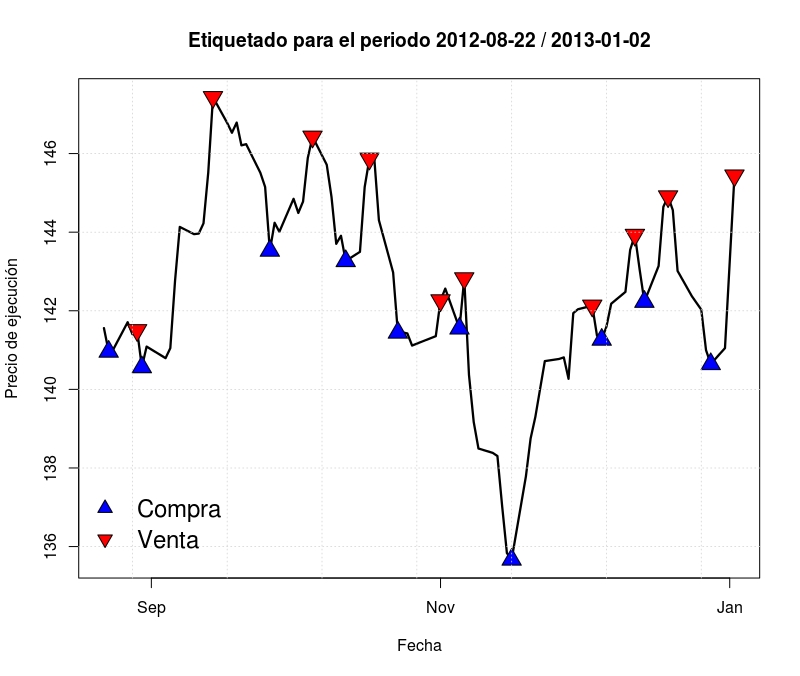
\includegraphics[width=1\linewidth]{imagenes/etiquetado.jpeg}}
\caption{\label{imagen:etiquetado} Resultado del proceso de etiquetado}
\end{figure}

\section{Atributos utilizados}
\label{seccion:atributos}
Los atributos utilizados en cada uno de los experimentos, son el conjunto de indicadores técnicos descritos en la sección \ref{subseccion:indicadores tecnicos}. Los parámetros utilizados para cada uno de ellos se describen a continuación, estos parámetros son los recomendados en la literatura del análisis técnico \cite{encycoplediaTechnicalIndicators}, \cite{technicalAnalysisKirkPatrick}.


\begin{itemize}
\item Oscilador Aroon con una ventana de tiempo de 25 días.

\item RSI con una ventana de tiempo de 14 días.

\item MFI con una ventana de tiempo de 14 días.

\item Williams \%R con una ventana de tiempo de 14 días.

\item CCI con una ventana de tiempo de 20 días.
\end{itemize}


\section{Aprendizaje incremental}
\label{seccion:aprendizaje incremental}
Tanto como para el algoritmo AQ como para el algoritmo CN2 se realizaron dos tipos de experimentos. El primero de ellos está basado en un enfoque de \textit{aprender-aplicar-descartar}, en el cual, dado un conjunto de entrenamiento, se induce un conjunto de reglas las cuales se aplican al conjunto de prueba más cercano. Después de esto, las reglas aprendidas se descartan (mecanismo de olvido).

El otro experimento se basa en un \textit{aprendizaje incremental}, en este caso, aprendemos un conjunto de reglas y en lugar de descartarlas, las ordenamos de acuerdo a su desempeño sobre el conjunto de entrenamiento del cual fueron inducidas por primera vez, así como su desempeño sobre los conjuntos de prueba en los cuales han sido aplicadas. En este enfoque mantenemos un conjunto de $k$-mejores reglas de compra y $k$-mejores reglas de venta.

Para medir el desempeño de las reglas sobre los conjuntos de entrenamiento de los cuales se inducen por primera vez, utilizamos la suma de su \textit{soporte} y su \textit{exactitud de Laplace}.

Por soporte, nos referimos al número de ejemplos de la clase positiva que cubre una regla, mientras que la exactitud de Laplace está dada por la ecuación (\ref{eqn:exactitud laplace})

\begin{equation}\label{eqn:exactitud laplace}
Exactitud\,de\,Laplace = \dfrac{ n_{c} + 1 }{ n_{tot} + k }
\end{equation}

en donde $n_c$ es el número de ejemplos de la clase $c$ que son cubiertos por la regla para esta misma clase, $n_{tot}$ es el número de ejemplos cubiertos por la regla y $k$ es el número de clases\footnote{Observemos que si una regla es consistente, entonces $n_c = n_{tot}$}.

Como se señala en \cite{CN2Improvements}, la exactitud de Laplace favorece el uso de reglas más generales sobre aquellas que son más específicas (elegidas al utilizar la exactitud clásica, $n_{c} / n_{tot} $). Consideremos el siguiente ejemplo para el caso con sólo dos clases:

\begin{itemize} 
\item Regla $R1$ cubre $1000$ ejemplos de la clase $C1$ y $1$ de la clase $C2$.

\item Regla $R2$ cubre $5$ ejemplos de la clase $C1$ y $0$ de la clase $C2$.
\end{itemize}

En este caso, la exactitud clásica de la regla $R2$ es igual a $100\%$, contra un $99\%$ de la regla $R1$, por lo tanto, a pesar de que esta última regla es más general que la primera, no le daríamos la preferencia que se le debería de dar. En cambio, utilizando la ecuación (\ref{eqn:exactitud laplace}), tenemos que la exactitud de Laplace para la regla $R1$  es aproximadamente $86\%$, mientras que para la regla $R2$ es de $99.8 \%$, con lo que capturamos el hecho de que esta última regla es más general.

Por otra parte, para medir el desempeño de las reglas sobre los conjuntos de prueba, primero las agrupamos en pares de \textit{compra-venta}. Estos pares de reglas se forman a partir de las señales de compra y venta generadas durante el periodo de prueba y son recompensadas (penalizadas) de acuerdo a la ganancia (pérdida) que generan.

Por ejemplo, consideremos un caso en el cual la regla de compra, $R_{C}$, nos indica que en el tiempo $t_1$ se debe de comprar, esta compra tendrá un precio de ejecución $P_{C}$. Conforme avanza el tiempo, notamos que la regla de venta, $R_{V}$, nos indica que en el tiempo $t_2 > t_1$, se debe de vender, esta venta tendrá precio de ejecución $P_{V}$. La recompensa (penalización) que se le asigna a cada regla en el par $\left(R_C, R_V\right)$ está dada por su ganancia (pérdida) porcentual, es decir:

\begin{equation}\label{eqn:recompensa reglas}
Recompensa(R_C, R_V) = \dfrac{P_V (1 - c)}{P_C (1 + c) } - 1
\end{equation}

en donde $c$ es el costo de transacción.

Finalmente, cada regla que no aparece en el conjunto de prueba que se está evaluando, se penaliza con la pérdida promedio que se tiene sobre este mismo conjunto de prueba; esto se utiliza como un mecanismo para ir descartando reglas debido al paso del tiempo.

De acuerdo a lo anterior, el puntaje de una regla $R$, antes de evaluar el conjunto de prueba $M$, está dado por:

\begin{equation} \label{eqn:puntaje de una regla}
puntaje_{-M}(R) = soporte(R) + Laplace(R) + \sum Recompensas
\end{equation}

en la ecuación (\ref{eqn:puntaje de una regla}), el término $ \sum Recompensas$ hace referencia a la suma de recompensas o penalizaciones que ha obtenido la regla $R$ para cada conjunto de prueba anterior al conjunto $M$.

De esta manera, ahora somos capaces de ordenar las reglas y por lo tanto acumular el aprendizaje así como identificar reglas útiles y descartar aquellas que no han funcionado.

La imagen \ref{imagen:aprendizaje_incremental} muestra el esquema del aprendizaje incremental que se propone en este trabajo.


\begin{figure}[ht]
\centering
\scalebox{1.0}{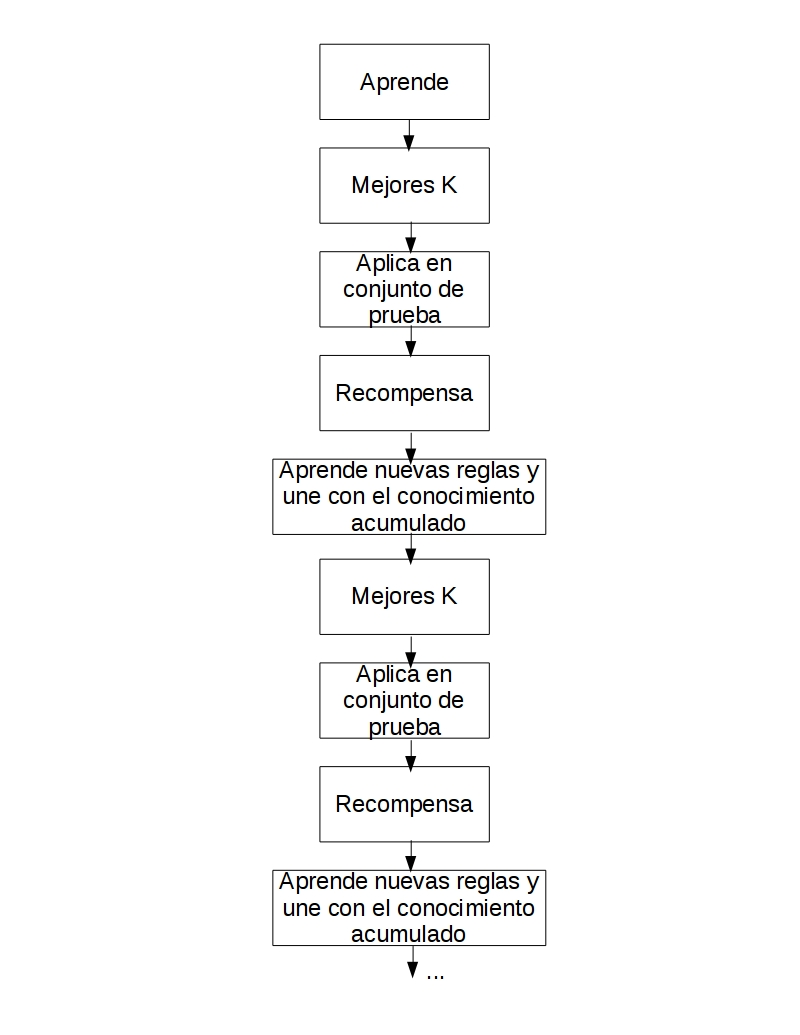
\includegraphics[width=1\linewidth]{imagenes/aprendizaje-incremental.jpg}}
\caption{\label{imagen:aprendizaje_incremental} Aprendizaje incremental}
\end{figure}


\section{Límites para las señales de venta}
\label{seccion:limites ventas}
Además de las reglas inducidas por cada algoritmo, utilizamos dos reglas adicionales las cuales buscan capturar el perfil de riesgo de los inversionistas.

Estas nuevas reglas establecen un límite superior (mercados a la alza) y un límite inferior (mercados a la baja) relativos a la última compra realizada. El primero de estos límites (límite superior) puede ser interpretado como el nivel de codicia o conformidad que tiene un inversionista, mientras que el segundo (límite inferior) se interpreta como el nivel de aversión al riesgo.

Utilizando estos límites y las reglas inducidas por cada algoritmo, una venta se ejecuta en dos etapas, llamaremos a la primera de ellas la etapa de la señal y a la segunda la etapa de confirmación.

En la etapa de la señal, para cada día $t$ (después del cierre del mercado), revisamos las reglas de venta en busca de una señal de venta de acuerdo a la información generada en este día. Si alguna regla nos dice que es un momento adecuado para vender, entonces pasamos a la etapa de confirmación.

En la etapa de confirmación, a lo largo del día de ejecución, $t_{ejec}$ (ver los supuestos de la sección \ref{sec:supuestos del mercado}), verificamos si la variación porcentual entre algún precio generado en este día, $P_{t_{ejec}}$ y el último precio al que compramos, $P_{C}^{ult}$, rebasa alguno de los límites establecidos.

Así pues, a través de estas dos etapas, se ejecuta una venta en el día $t_{ejec}$ si alguna de las siguientes condiciones se cumple:

\begin{align}
R_{venta}(t) \wedge (Var(t_{ejec}, P_{t_{ejec}}, P_{C}^{ult} ) > LS) \label{eqn:Venta limite sup}\\
R_{venta}(t) \wedge (Var(t_{ejec}, P_{t_{ejec}}, P_{C}^{ult} ) < LI) \label{eqn:Venta limite inf}
\end{align}

en donde $R_{venta}(t)$ representa una regla de venta inducida por los algoritmos AQ o CN2, la cual es aplicada a la información del día $t$, $LS>0$ es el límite superior expresado como un porcentaje relativo al último precio de compra, $LI<0$ es el límite inferior expresado como un porcentaje relativo al último precio de compra y $Var(t_{ejec}, P_{t_{ejec}}, P_{C}^{ult} )$ representa la variación porcentual entre los precios generados a lo largo del día $t_{ejec}$, $P_{t_{ejec}}$, respecto al último precio de compra, $P_{C}^{ult}$, como se muestra en la ecuación (\ref{eqn:variacion bandas})

\begin{equation} \label{eqn:variacion bandas}
Var(t_{ejec}, P_{t_{ejec}}, P_{C}^{ult} ) = \dfrac{P_{t_{ejec}}} {P_{C}^{ult}} - 1
\end{equation}

La imagen \ref{imagen:bandas horizontales} muestra un ejemplo de los límites relativos a una señal de compra.

\begin{figure}[htbp]
\centering
\scalebox{0.8}{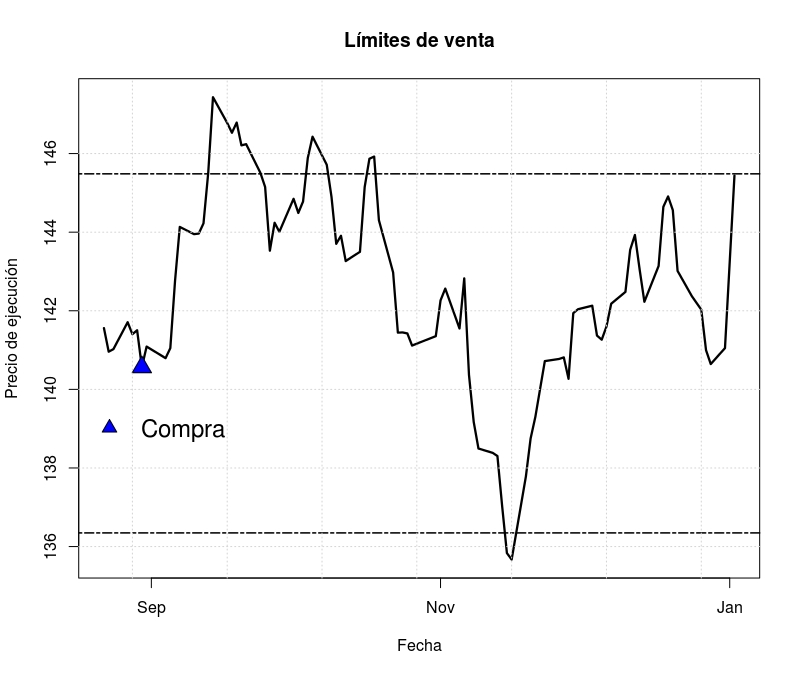
\includegraphics[width=1\linewidth]{imagenes/bandas_horizontales.jpeg}}
\caption{\label{imagen:bandas horizontales} Límites para las señales de venta relativos a una señal de compra}
\end{figure}

\section{Supuestos del mercado}
\label{sec:supuestos del mercado}
Para cada experimento, se consideraron los siguientes supuestos:

\begin{itemize}
\item El precio de ejecución en el día $t$ será el promedio entre el precio máximo y el precio mínimo de ese día.

\item Dada una señal de compra o venta en el día $t$, la acción se ejecuta en el día $t+1$ utilizando el precio de ejecución.

\item El costo de cada transacción se fija en $0.25\%$. Así para cada compra con precio de ejecución $P_{C}$ terminamos pagando un total de 
$$P_{C}(1 + 0.0025)$$
por cada acción comprada.

De la misma forma, por cada acción que vendemos a un precio $P_{V}$, recibimos 
$$P_{V}(1 - 0.0025)$$

\item En cada señal de compra, compramos tantas acciones podamos comprar con nuestro capital disponible (considerando el costo de transacción).

\item Para cada señal de venta, vendemos todas las acciones que poseemos.

\item Sólo podemos vender cuando tenemos acciones en nuestra posesión, es decir, no se permiten ventas en corto.

\item El límite superior para las señales de venta, $LS$, se fija con un valor de $0.035$ o $3.5\%$ relativo al último precio de compra.

\item El límite inferior para las señales de venta, $LI$, se fija con un valor de $-0.03$ o $-3.0\%$ relativo al último precio de compra.

\item El capital inicial es de $\$100,000$ unidades monetarias (pesos en el caso del NAFTRAC y dólares de Estados Unidos para el SPDR S\&P 500).
\end{itemize}

%=============== Resultados ================= %
\chapter[Capítulo \thechapter: Resultados experimentales]{Resultados experimentales}
\label{capitulo:resultados experimentales}
Utilizando la metodología descrita en el capítulo \ref{capitulo:solucion propuesta}, para cada TRAC (ver sección \ref{seccion:indices accionarios}) se realizaron cuatro experimentos distintos. Estos experimentos exploran dos alternativas distintas para discretizar los atributos continuos, \cite{dataMiningUsingR}, así como el tipo de aprendizaje aplicado (incremental o no incremental).

El primero de los métodos de discretización (al cual denotaremos como DI), se basa en crear intervalos con el mismo tamaño, sin importar la distribución de los valores de cada atributo; por otro lado, el segundo método (denotado como DC) utiliza los cuantiles de cada atributo con el fin de crear intervalos equiprobables.

Así pues, tenemos los siguiente experimentos:

\begin{itemize}
\item Aprendizaje incremental con discretización por intervalos de mismo tamaño (AI-DI).

\item Aprendizaje no incremental con discretización por intervalos de mismo tamaño (AN-DI).

\item Aprendizaje incremental con discretización por cuantiles (AI-DC).

\item Aprendizaje no incremental con discretización por cuantiles (AN-DC).

\end{itemize}

\section{Resultados para el SPDR S\&P 500}
\label{seccion:resultados sp500}
Las tablas \ref{tabla:AQ-SP500} y \ref{tabla:CN2-SP500}, muestran un resumen de los resultados obtenidos en los $30$ conjuntos de prueba con la información del SPDR S\&P 500.


\begin{center}
\begin{table}[htbp]
\centering
\begin{tabular}{ccccc}
\hline
\textbf{AQ} & \textbf{AI-DI} & \textbf{AN-DI} & \textbf{AI-DC} & \textbf{AN-DC} \\
\hline
Exceso de ganancia promedio & $0.37\%$ & $-0.39\%$ & $0.20\%$ & $-1.02\%$ \\
Casos mejores que \textit{compra y espera} & $11$ & $14$ & $10$ & $13$  \\
Casos peores que \textit{compra y espera} & $19$ & $16$ & $20$ & $17$ \\
Exceso de ganancia máximo & $34.64\%$ & $22.17\%$ & $29.72\%$ & $20.3\%$ \\
Exceso de ganancia mínimo & $-11.23\%$ & $-12.94\%$ & $-3.86\%$ & $-11.47\%$ \\
Ganancia monetaria promedio & $\$2,384.18$ & $\$1,620.11$ & $\$2,214.84$ & $\$ 994.96$ \\
\hline
\end{tabular}
\caption{\label{tabla:AQ-SP500} Resultados del algoritmo AQ para el SPDR S\&P 500}
\end{table}
\end{center}


\begin{center}
\begin{table}[htbp]
\centering
\begin{tabular}{ccccc}
\hline
\textbf{CN2} & \textbf{AI-DI} & \textbf{AN-DI} & \textbf{AI-DC} & \textbf{AN-DC} \\
\hline
Exceso de ganancia promedio & $-1.22\%$ & $-1.07\%$ & $-0.54\%$ & $-1.41\%$ \\
Casos mejores que \textit{compra y espera} & $11$ & $10$ & $12$ & $8$  \\
Casos peores que \textit{compra y espera} & $19$ & $20$ & $18$ & $22$ \\
Exceso de ganancia máximo & $15.69\%$ & $12.32\%$ & $11.81\%$ & $6.05\%$ \\
Exceso de ganancia mínimo & $-12.87\%$ & $-9.43\%$ & $-6.48\%$ & $-8.33\%$ \\
Ganancia monetaria promedio & $\$792.43$ & $\$946.07$ & $\$1,475.04$ & $\$ 604.99$ \\

\hline
\end{tabular}
\caption{\label{tabla:CN2-SP500}Resultados del algoritmo CN2 para el SPDR S\&P 500}
\end{table}
\end{center}

Como se observa en la tabla \ref{tabla:AQ-SP500}, para el algortimo AQ, el aprendizaje incremental resulta superior al no incremental en ambos métodos de discretización, obteniendo un exceso de ganancia promedio positivo (aunque muy pequeño).

Por otro lado, como se muestra en la tabla \ref{tabla:CN2-SP500}, el algoritmo CN2 se desempeña pobremente en todos los experimentos, aunque se obtiene el mejor resultado utilizando un algoritmo de aprendizaje incremental.

\begin{figure}[htbp]
\centering
\scalebox{0.8}{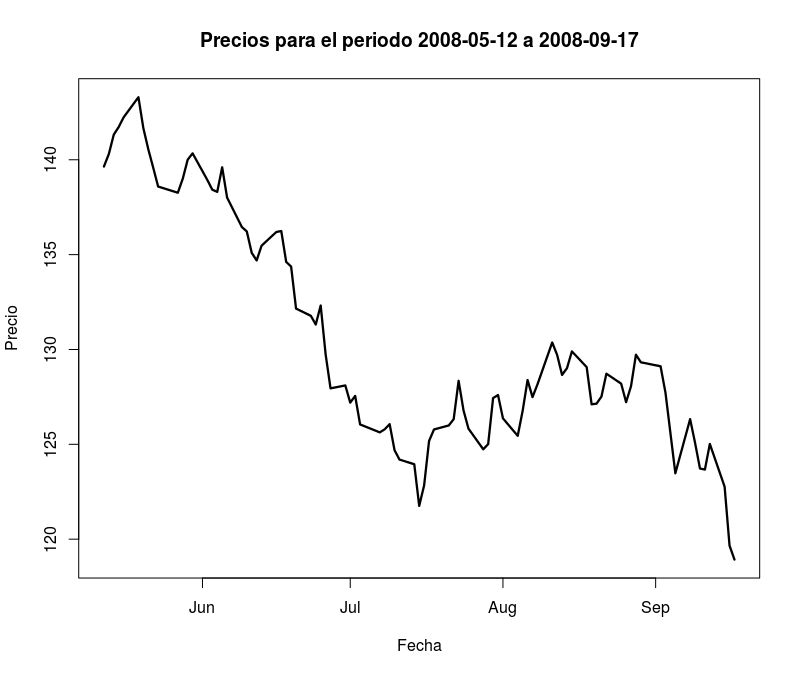
\includegraphics[width=1\linewidth]{imagenes/sp500-2008-05-12.jpeg}}
\caption{\label{imagen:sp500-2008-05-12} Gráfica del precio del SPDR S\&P 500, 2008/05/12 - 2008/09/17}
\end{figure}

Es importante señalar que estamos considerando dos periodos correspondientes a la crisis financiera de 2008\footnote{Crisis hipotecaria en Estados Unidos}, como se ilustra en las imágenes \ref{imagen:sp500-2008-05-12} y \ref{imagen:sp500-2008-09-18}, durante estos periodos el precio mostró una fuerte tendencia a la baja, en consecuencia, superar la ganancia de la estrategia \textit{compra y espera} no implica reto alguno como se puede constatar analizando las tablas \ref{tabla:AQ-SP500-2008} y \ref{tabla:CN2-SP500-2008}. Con estas tablas y las tablas \ref{tabla:AQ-SP500} y \ref{tabla:CN2-SP500}, podemos comprobar que, en la mayoría de los casos, el exceso de ganancia máximo corresponde precisamente a estos periodos.

\begin{figure}[htbp]
\centering
\scalebox{0.8}{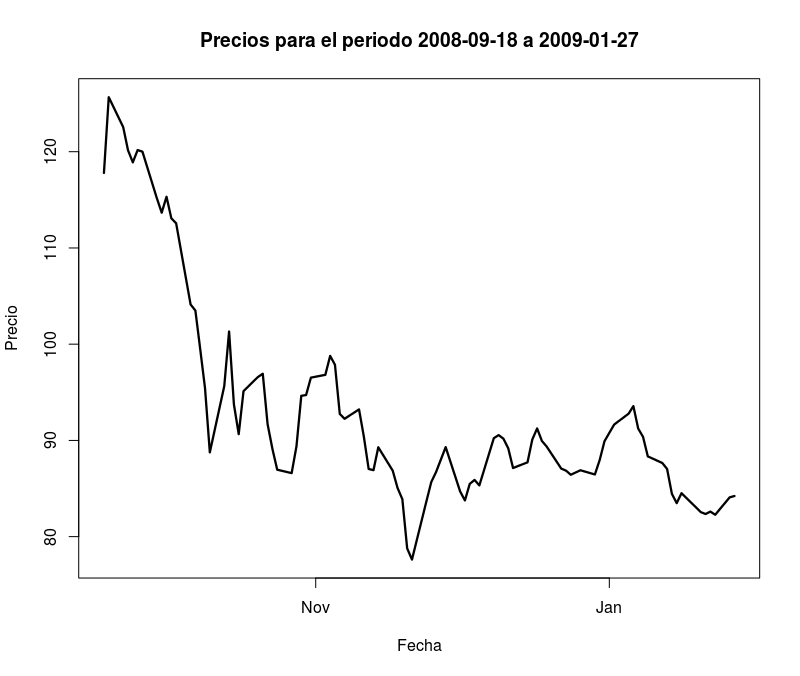
\includegraphics[width=1\linewidth]{imagenes/sp500-2008-09-18.jpeg}}
\caption{\label{imagen:sp500-2008-09-18} Gráfica del precio del SPDR S\&P 500, 2008/09/18 - 2009/01/27}
\end{figure}

\begin{center}
\begin{table*}[htbp]
\centering
\begin{tabular}{ccccc}
\hline
\textbf{AQ periodo 2008} & \textbf{AI-DI} & \textbf{AN-DI} & \textbf{AI-DC} & \textbf{AN-DC} \\
\hline
$2008/05/12$ - $2008/09/17$ & $8.13\%$ & $2.33\%$ & $6.14\%$ & $3.57\%$ \\
$2008/09/18$ - $2009/01/27$ & $34.64\%$ & $22.17\%$ & $29.72\%$ & $20.37	\%$  \\
\hline
\end{tabular}
\caption{\label{tabla:AQ-SP500-2008} Exceso de ganancia del algoritmo AQ en la crisis financiera de 2008}
\end{table*}
\end{center}

\begin{center}
\begin{table*}[htbp]
\centering
\begin{tabular}{ccccc}
\hline
\textbf{CN2 periodo 2008} & \textbf{AI-DI} & \textbf{AN-DI} & \textbf{AI-DC} & \textbf{AN-DC} \\
\hline
$2008/05/12$ - $2008/09/17$ & $0.27\%$ & $-0.38\%$ & $5.06\%$ & $-2.81\%$ \\
$2008/09/18$ - $2009/01/27$ & $15.69\%$ & $12.32\%$ & $11.81\%$ & $-0.62\%$  \\
\hline
\end{tabular}
\caption{\label{tabla:CN2-SP500-2008} Exceso de ganancia del algoritmo CN2 en la crisis financiera de 2008}
\end{table*}
\end{center}

Así pues, como se señala en \cite{Lohpetch2010}, el verdadero desafío se encuentra en superar a la estrategia \textit{compra y espera} en mercados con una tendencia alcista en los precios. Por lo tanto, calculamos el desempeño de cada algoritmo únicamente en periodos en donde se hace presente este tipo de tendencia. En total se detectaron 16 periodos con tendencia a la alza, los resultados se muestran en las tablas \ref{tabla:AQ-SP500-alza} y \ref{tabla:CN2-SP500-alza}.

\begin{center}
\begin{table}[htbp]
\centering
\begin{tabular}{ccccc}
\hline
\textbf{AQ periodos a la alza} & \textbf{AI-DI} & \textbf{AN-DI} & \textbf{AI-DC} & \textbf{AN-DC} \\
\hline
Exceso de ganancia promedio & $-0.85\%$ & $-2.07\%$ & $-0.59\%$ & $-2.39\%$ \\
Casos mejores que \textit{compra y espera} & $5$ & $5$ & $6$ & $5$  \\
Casos peores que \textit{compra y espera} & $11$ & $11$ & $10$ & $11$ \\
Exceso de ganancia máximo & $2.33\%$ & $3.86\%$ & $2.30\%$ & $0.85\%$ \\
Exceso de ganancia mínimo & $-3.83\%$ & $-12.94\%$ & $-3.85\%$ & $-11.47\%$ \\
Ganancia monetaria promedio & $\$7,051.72$ & $\$5,830.17$ & $\$7,312.90$ & $\$5,514.90$ \\
\hline
\end{tabular}
\caption{\label{tabla:AQ-SP500-alza}Resultados del algoritmo AQ para el SPDR S\&P 500 en periodos a la alza}
\end{table}
\end{center}


\begin{center}
\begin{table}[htbp]
\centering
\begin{tabular}{ccccc}
\hline
\textbf{CN2 periodos a la alza} & \textbf{AI-DI} & \textbf{AN-DI} & \textbf{AI-DC} & \textbf{AN-DC} \\
\hline
Exceso de ganancia promedio & $-2.55\%$ & $-1.84\%$ & $-1.28\%$ & $-2.37\%$ \\
Casos mejores que \textit{compra y espera} & $5$ & $6$ & $6$ & $3$  \\
Casos peores que \textit{compra y espera} & $11$ & $10$ & $10$ & $13$ \\
Exceso de ganancia máximo & $0.52\%$ & $9.52\%$ & $1.00\%$ & $0.80\%$ \\
Exceso de ganancia mínimo & $-12.87\%$ & $-9.43\%$ & $-6.48\%$ & $-8.33\%$ \\
Ganancia monetaria promedio & $\$5,346.94$ & $\$6,059.76$ & $\$6,624.75$ & $\$5,529.46$ \\
\hline
\end{tabular}
\caption{\label{tabla:CN2-SP500-alza}Resultados del algoritmo CN2 para el SPDR S\&P 500 en periodos a la alza}
\end{table}
\end{center}

De acuerdo a estas tablas, en ningún caso los algoritmos fueron capaces de vencer a la estrategia \textit{compra y espera}. Sin embargo, nuevamente para el algoritmo AQ los mejores resultados se obtienen con un aprendizaje incremental.

\section{Resultados para el NAFTRAC}
\label{seccion:resultados NAFTRAC}
Analizando los 15 conjuntos de prueba con la información del NAFTRAC obtenemos los resultados de las tablas  \ref{tabla:AQ-NAFTRAC} y \ref{tabla:CN2-NAFTRAC}.

\begin{center}
\begin{table}[h]
\centering
\begin{tabular}{ccccc}
\hline
\textbf{AQ} & \textbf{AI-DI} & \textbf{AN-DI} & \textbf{AI-DC} & \textbf{AN-DC} \\
\hline
Exceso de ganancia promedio & $1.29\%$ & $0.13\%$ & $0.59\%$ & $-0.30\%$ \\
Casos mejores que \textit{compra y espera} & $11$ & $8$ & $9$ & $7$  \\
Casos peores que \textit{compra y espera} & $14$ & $7$ & $6$ & $8$ \\
Exceso de ganancia máximo & $6.74\%$ & $5.16\%$ & $4.60\%$ & $1.85\%$ \\
Exceso de ganancia mínimo & $-6.78\%$ & $-6.27\%$ & $-3.44\%$ & $-3.46\%$ \\
Ganancia monetaria promedio & $\$1,697.77$ & $\$530.62$ & $\$993.49$ & $\$103.29$ \\
\hline
\end{tabular}
\caption{\label{tabla:AQ-NAFTRAC} Resultados del algoritmo AQ para el NAFTRAC}
\end{table}
\end{center}

\begin{center}
\begin{table}[h]
\centering
\begin{tabular}{ccccc}
\hline
\textbf{CN2} & \textbf{AI-DI} & \textbf{AN-DI} & \textbf{AI-DC} & \textbf{AN-DC} \\
\hline
Exceso de ganancia promedio & $-0.68\%$ & $0.17\%$ & $0.20\%$ & $0.06\%$ \\
Casos mejores que \textit{compra y espera} & $7$ & $10$ & $8$ & $9$  \\
Casos peores que \textit{compra y espera} & $8$ & $5$ & $7$ & $6$ \\
Exceso de ganancia máxima & $3.41\%$ & $4.33\%$ & $4.60\%$ & $4.00\%$ \\
Exceso de ganancia mínimo & $-4.87\%$ & $-6.00\%$ & $-3.44\%$ & $-6.46\%$ \\
Ganancia monetaria promedio & $\$-273.29$ & $\$578.85$ & $\$602.01$ & $\$461.66$ \\
\hline
\end{tabular}
\caption{\label{tabla:CN2-NAFTRAC} Resultados del algoritmo CN2 para el NAFTRAC}
\end{table}
\end{center}

De la misma forma que en los experimentos anteriores, el algoritmo AQ con aprendizaje incremental obtiene los mejores resultados para cada método de discretización, mientras que el algoritmo CN2 nuevamente presenta un desempeño pobre.

Enfocándonos en los periodos a la alza (se detectaron un total de 7 periodos con esta tendencia), como se muestra en las tablas \ref{tabla:AQ-NAFTRAC-alza} y \ref{tabla:CN2-NAFTRAC-alza} ambos algoritmos fueron capaces de vencer a la estrategia \textit{compra y espera} en 3 de 4 experimentos, obteniéndose el mejor resultado con el algoritmo AQ utilizando un aprendizaje incremental y una discretización basada en cuantiles.

\begin{center}
\begin{table}[h]
\centering
\begin{tabular}{ccccc}
\hline
\textbf{AQ periodos a la alza} & \textbf{AI-DI} & \textbf{AN-DI} & \textbf{AI-DC} & \textbf{AN-DC} \\
\hline
Exceso de ganancia promedio & $0.18\%$ & $0.87\%$ & $1.54\%$ & $-0.07\%$ \\
Casos mejores que \textit{compra y espera} & $4$ & $4$ & $5$ & $5$  \\
Casos peores que \textit{compra y espera} & $3$ & $3$ & $2$ & $2$ \\
Exceso de ganancia máximo & $5.03\%$ & $5.16\%$ & $4.60\%$ & $1.39\%$ \\
Exceso de ganancia mínimo & $-6.78\%$ & $-2.68\%$ & $-2.86\%$ & $-3.20\%$ \\
Ganancia monetaria promedio & $\$5,201.07$ & $\$5,895.67$ & $\$6,562.47$ & $\$4,950.47$ \\
\hline
\end{tabular}
\caption{\label{tabla:AQ-NAFTRAC-alza} Resultados del algoritmo AQ para el NAFTRAC en periodos a la alza}
\end{table}
\end{center}

\begin{center}
\begin{table}[htbp]
\centering
\begin{tabular}{ccccc}
\hline
\textbf{CN2 periodos a la alza} & \textbf{AI-DI} & \textbf{AN-DI} & \textbf{AI-DC} & \textbf{AN-DC} \\
\hline
Exceso de ganancia promedio & $-0.42\%$ & $1.06\%$ & $0.27\%$ & $0.87\%$ \\
Casos mejores que \textit{compra y espera} & $4$ & $6$ & $4$ & $5$  \\
Casos peores que \textit{compra y espera} & $3$ & $1$ & $3$ & $2$ \\
Exceso de ganancia máximo & $2.98\%$ & $3.91\%$ & $4.60\%$ & $4.00\%$ \\
Exceso de ganancia mínimo & $-3.11\%$ & $-0.77\%$ & $-3.11\%$ & $-1.45\%$ \\
Ganancia monetaria promedio & $\$4,605.01$ & $\$6,079.97$ & $\$5,294.73$ & $\$5,892.17$ \\
\hline
\end{tabular}
\caption{\label{tabla:CN2-NAFTRAC-alza} Resultados del algoritmo CN2 para el NAFTRAC en periodos a la alza}
\end{table}
\end{center}



%=============== Conclusión ================= %
\chapter[Capítulo \thechapter: Conclusiones y trabajo futuro]{Conclusiones y trabajo futuro}
\label{capitulo:conclusiones}
%Las reglas aprendidas tienen sentido financiero?
%Aprendizaje incremental no es apropiado para CN2 pero si para AQ
\section{Conclusiones}
\label{seccion:conclusiones}
De acuerdo a los resultados de la sección \ref{capitulo:resultados experimentales}, tanto como para el mercado mexicano como para el estadounidense, el algoritmo AQ con aprendizaje incremental, es superior a cualquier versión del algoritmo CN2. Más aún, para el caso del mercado mexicano, este algoritmo logra vencer (en promedio) a la estrategia \textit{compra y espera} aún en mercados que presentan una tendencia a la alza. 

Es importante señalar que, a pesar de que no siempre vencemos a la estrategia \textit{compra y espera}, únicamente en un caso obtuvimos una ganancia monetaria promedio negativa (algoritmo CN2 experimento AI-DI, tabla \ref{tabla:CN2-NAFTRAC}), en el resto de los experimentos, en promedio, no perdemos dinero, una característica claramente deseable para cualquier algoritmo de inversión.

Finalmente, desde el punto de vista de la teoría económica, nuestros resultados experimentales indican que el mercado mexicano es menos eficiente que el mercado estadounidense. Esto está en línea con lo que se expone en \cite{CFA2019}, en donde se señala que uno de los factores que contribuye a la eficiencia del mercado, es el número de participantes que hay en este (a mayor número de participantes, mayor eficiencia hay).

\section{Trabajo futuro}
\label{seccion:trabajo futuro}
%¿Como establecer las bandas horizontales?
%Parámetros de los indicadores técnicos
%Medida de riesgo
%Otras formas de dar puntajes de las reglas
%Supuestos del precio de ejecución
%Otros atributos
%Incorporar información relativa a la versión semifuerte de la HME
Entre las posibles líneas de extensión de este trabajo, se encuentran:

\begin{itemize}
\item Incorporar otro tipo de información pública, esto es, extender este trabajo con el fin de vencer la versión semifuerte de la hipótesis del mercado eficiente.

\item Idear una metodología para saber la proporción de dinero a invertir en cada señal de compra y no invertir todo el capital disponible.

\item Investigar el uso de otros indicadores técnicos, así como los parámetros de estos.

\item Analizar el desempeño de las estrategias considerando alguna medida de riesgo utilizada las finanzas.

\item Investigar la posición óptima para los límites de las señales de venta.

\item Probar con datos en escalas de tiempo más finas, por ejemplo, datos de cada 5 minutos.
\end{itemize}


\bibliography{references}
\addcontentsline{toc}{chapter}{Referencias}

%no citados en antecedentes ya que se desvían de la metodología propuesta pero fueron consultados para obtener un panorama más ámplio
\nocite{Preen2010}
\nocite{Kuo2013}
\nocite{Wang2014}
\nocite{Hu2015} %artículo de revisión de la literatura


\end{document}